\section{Células diádicas e operador gerador}
\label{sec:generator}

\subsection{Células, posse e centros}

Para $k\in\Nzero$ e $m\in\mathbb{Z}$, sejam
\begin{equation}
 J_{k,m}=[m2^{-k},(m+1)2^{-k}],\qquad
 J_{k,m}^{\own}=[m2^{-k},(m+1)2^{-k}),
 \label{eq:dyadic-cells}
\end{equation}
e
\begin{equation}
 x_0(k,m)=\left(m+\frac12\right)2^{-k}=\frac{2m+1}{2^{k+1}}.
 \label{eq:dyadic-center}
\end{equation}
A célula fechada sustenta o segmento; a versão semiaberta atribui cada fronteira a um único proprietário. Escreva
\[
 \mathbb{D}=\{j2^{-K}:j\in\mathbb{Z},\ K\in\Nzero\},\qquad
 \Dmid=\mathbb{D}\setminus\mathbb{Z}.
\]

\begin{lemma}[estrutura diádica]\label{lem:dyadic}
Para cada $k$, as células $J_{k,m}^{\own}$ particionam $\mathbb{R}$ e
\begin{equation}
 J_{k,m}=J_{k+1,2m}\cup J_{k+1,2m+1},\qquad |J_{k,m}|=2^{-k}.
 \label{eq:refinement}
\end{equation}
O mapa $(k,m)\mapsto x_0(k,m)$ é uma bijeção de $\Nzero\times\mathbb{Z}$ sobre $\Dmid$, que é denso em $\mathbb{R}$.
\end{lemma}

\begin{proof}
Para $x\in\mathbb{R}$, o único índice de posse na escala $k$ é $m=\lfloor2^kx\rfloor$; isso prova a partição. A identidade de refinamento decorre de cindir $[2m2^{-(k+1)},(2m+2)2^{-(k+1)}]$ em seu ponto médio.

Pela \eqref{eq:dyadic-center}, o centro tem numerador ímpar e denominador reduzido $2^{k+1}\ge2$, logo pertence a $\Dmid$. Reciprocamente, cada $x\in\Dmid$ possui forma reduzida única $j/2^K$, com $K\ge1$ e $j$ ímpar; tomando $k=K-1$ e $m=(j-1)/2$, obtém-se $x=x_0(k,m)$. A mesma unicidade prova a injetividade. Por fim, os centros de escala $k$ estão espaçados por $2^{-k}$; escolhendo o mais próximo de um real dado, a distância tende a zero com $k$, o que prova a densidade.
\end{proof}

A convenção de posse, os centros e o primeiro passo de refinamento aparecem
esquematicamente na \cref{fig:dyadic-pt}.

\begin{figure}[t]
 \centering
 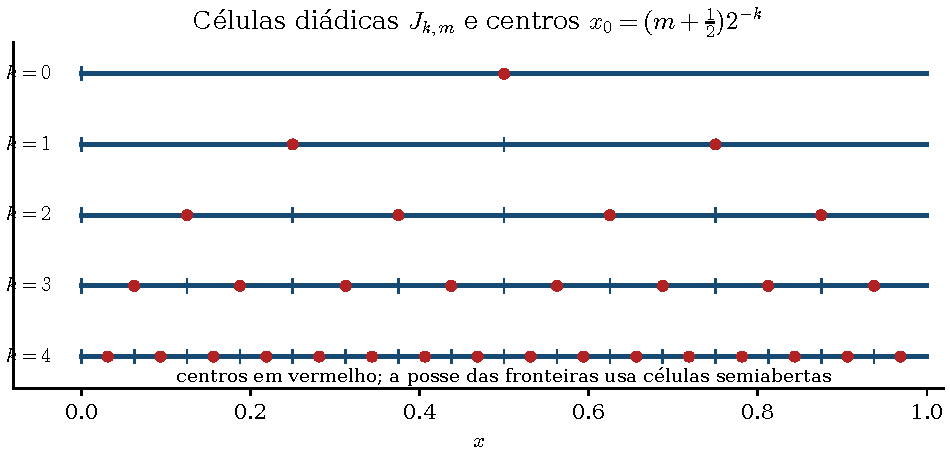
\includegraphics[width=.91\linewidth]{fig01_diadicos.pdf}
 \caption{Células diádicas, centros e convenção semiaberta de posse.}
 \label{fig:dyadic-pt}
\end{figure}

\subsection{Retas ancoradas e descompactação}

Dados $x_0,y_0\in\mathbb{R}$ e $s\neq0$, a reta ancorada é
\begin{equation}
 \ell(x)=y_0+s(x-x_0)=a+bx,\qquad b=s,\quad a=y_0-sx_0.
 \label{eq:anchored-line}
\end{equation}
Para $n\in\Nzero$, aplique sucessivamente a inversa do pareamento:
\begin{equation}
 (u,v)=\pi^{-1}(n),\qquad (k,\mu)=\pi^{-1}(u),\qquad (r,t)=\pi^{-1}(v).
 \label{eq:unpack}
\end{equation}

\begin{lemma}\label{lem:unpack}
O mapa $n\mapsto(k,\mu,r,t)$ de \eqref{eq:unpack} é uma bijeção de $\Nzero$ sobre $\Nzero^4$.
\end{lemma}

\begin{proof}
Sua inversa explícita é
\[
 (k,\mu,r,t)\longmapsto \pi\bigl(\pi(k,\mu),\pi(r,t)\bigr),
\]
uma composição de bijeções pelo \cref{lem:cantor}.
\end{proof}

Defina
\begin{equation}
 m=Z(\mu),\quad x_{0,n}=x_0(k,m),\quad y_{0,n}=Q(r),\quad s_n=Q^{\!*}(t),
 \label{eq:local-parameters}
\end{equation}
e converta para a forma global por
\begin{equation}
 b_n=s_n,\qquad a_n=y_{0,n}-s_nx_{0,n}.
 \label{eq:global-parameters}
\end{equation}
Se $x_L=m2^{-k}$ e $x_R=(m+1)2^{-k}$, ponha
\begin{equation}
 c_n=\min\{\ell_n(x_L),\ell_n(x_R)\},\qquad
 d_n=\max\{\ell_n(x_L),\ell_n(x_R)\}.
 \label{eq:range}
\end{equation}

\begin{definition}[gerador e biblioteca]\label{def:generator}
Se $\Intervals$ é o conjunto dos intervalos fechados não degenerados de $\mathbb{R}$, defina
\begin{equation}
 \Gamma:\Nzero\to\mathbb{R}\times(\mathbb{R}\setminus\{0\})\times\Intervals,
 \qquad \Gamma(n)=(a_n,b_n,[c_n,d_n]).
 \label{eq:generator}
\end{equation}
A biblioteca é $\Library=\Gamma(\Nzero)$. O átomo de endereço $n$ é a restrição de $\ell_n$ à célula $J_{k(n),m(n)}$.
\end{definition}

Como $s_n\neq0$ e $x_L\neq x_R$, o intervalo em \eqref{eq:range} é não degenerado, de modo que \eqref{eq:generator} está bem definido.

A exclusão da inclinação nula é estrutural, e não apenas uma convenção de
parametrização. É precisamente $b_n\neq0$ que torna a interface global
invertível no eixo espacial e permite recuperar a célula pela fórmula
\eqref{eq:preimage-intro}. Se fossem admitidas peças constantes, a imagem
$[c_n,d_n]$ degeneraria em um ponto e deixaria de codificar o intervalo de
origem. A extensão marcada $\Library^\square$, introduzida na
\cref{sec:regularized-reversibility}, é usada somente como dispositivo auxiliar
em resultados de reversão que precisam representar regiões planas; ela não
substitui a biblioteca original $\Library$ nem sua semântica de endereçamento.

Para uma interface global $\Gamma(n)=(a_n,b_n,[c_n,d_n])$, defina sua
pré-imagem espacial por
\begin{equation}
 I_n^x=\left[
 \min\!\left\{\frac{c_n-a_n}{b_n},\frac{d_n-a_n}{b_n}\right\},
 \max\!\left\{\frac{c_n-a_n}{b_n},\frac{d_n-a_n}{b_n}\right\}
 \right].
 \label{eq:preimage-intro}
\end{equation}

\subsection{Recuperação da célula e endereço canônico}

\begin{lemma}[validade espacial exata]\label{lem:cell-recovery}
Para todo $n\in\Nzero$, o intervalo $I_n^x$ definido em \eqref{eq:preimage-intro} satisfaz
\[
 I_n^x=J_{k(n),m(n)}.
\]
\end{lemma}

\begin{proof}
Como $b_n\neq0$, $\ell_n$ é uma bijeção afim estritamente monótona. Sua restrição a $[x_L,x_R]$ tem imagem $[c_n,d_n]$ por \eqref{eq:range}; logo $\ell_n^{-1}([c_n,d_n])=[x_L,x_R]$. Os dois quocientes em \eqref{eq:preimage-intro} são precisamente $\ell_n^{-1}(c_n)$ e $\ell_n^{-1}(d_n)$, possivelmente em ordem invertida quando $b_n<0$.
\end{proof}

\begin{theorem}[unicidade do endereço]\label{thm:injective}
$\Gamma$ é injetiva. Portanto, é uma bijeção de $\Nzero$ sobre $\Library$ e cada átomo tem um único endereço.
\end{theorem}

\begin{proof}
Suponha $\Gamma(n)=\Gamma(n')=(a,b,[c,d])$. Por \cref{lem:cell-recovery}, a tripla recupera a célula comum $J=[x_L,x_R]$. Seu comprimento determina unicamente $k=-\log_2|J|$, e $m=2^kx_L$. Assim, também se recupera $x_0=(m+1/2)2^{-k}$. A inclinação local é $s=b$ e o valor ancorado é $y_0=a+bx_0$.

Pelas bijeções dos \cref{lem:dyadic,lem:integers,lem:rational-rank}, os dados $(x_0,y_0,s)$ determinam unicamente $(k,\mu,r,t)$. O \cref{lem:unpack} determina então um único $n$. Logo $n=n'$.
\end{proof}

Em uma fronteira, duas células fechadas podem estar ativas. A célula semiaberta escolhe uma proprietária; em uma montagem contínua, as duas peças têm o mesmo valor no nó e essa escolha não altera a função.

\begin{theorem}[dicionário de jatos racionais]\label{thm:dictionary}
O mapa
\begin{equation}
 n\longmapsto(x_{0,n},y_{0,n},s_n)
 \label{eq:dictionary}
\end{equation}
é uma bijeção de $\Nzero$ sobre $\Dmid\times\mathbb{Q}\times\Qstar$. Sua imagem é densa em $\mathbb{R}^3$.
\end{theorem}

\begin{proof}
A bijetividade resulta da composição das bijeções em \eqref{eq:unpack}--\eqref{eq:local-parameters}. A densidade decorre da densidade de $\Dmid$, de $\mathbb{Q}$ e de $\Qstar$ em $\mathbb{R}$, aplicada coordenada a coordenada na norma do máximo.
\end{proof}

O dicionário \eqref{eq:dictionary} parametriza todos os 1-jatos com centro
diádico não inteiro, valor racional e derivada racional não nula. A
aproximação global resulta das montagens contínuas desses dados locais,
introduzidas na seção seguinte.
